\section{Sonuçlar}
Bu bölümde eğitim dinamikleri, nicel test sonuçları, nitel örnekler ve damar analizi bulguları sunulmaktadır.

\subsection{Eğitim ve Doğrulama Eğrileri}
Şekil~\ref{fig:trainloss} eğitim kaybı (loss) değişimini, Şekil~\ref{fig:valmetrics} doğrulama metriklerinin epoch'lara göre değişimini göstermektedir.

\begin{figure}[H]
\centering
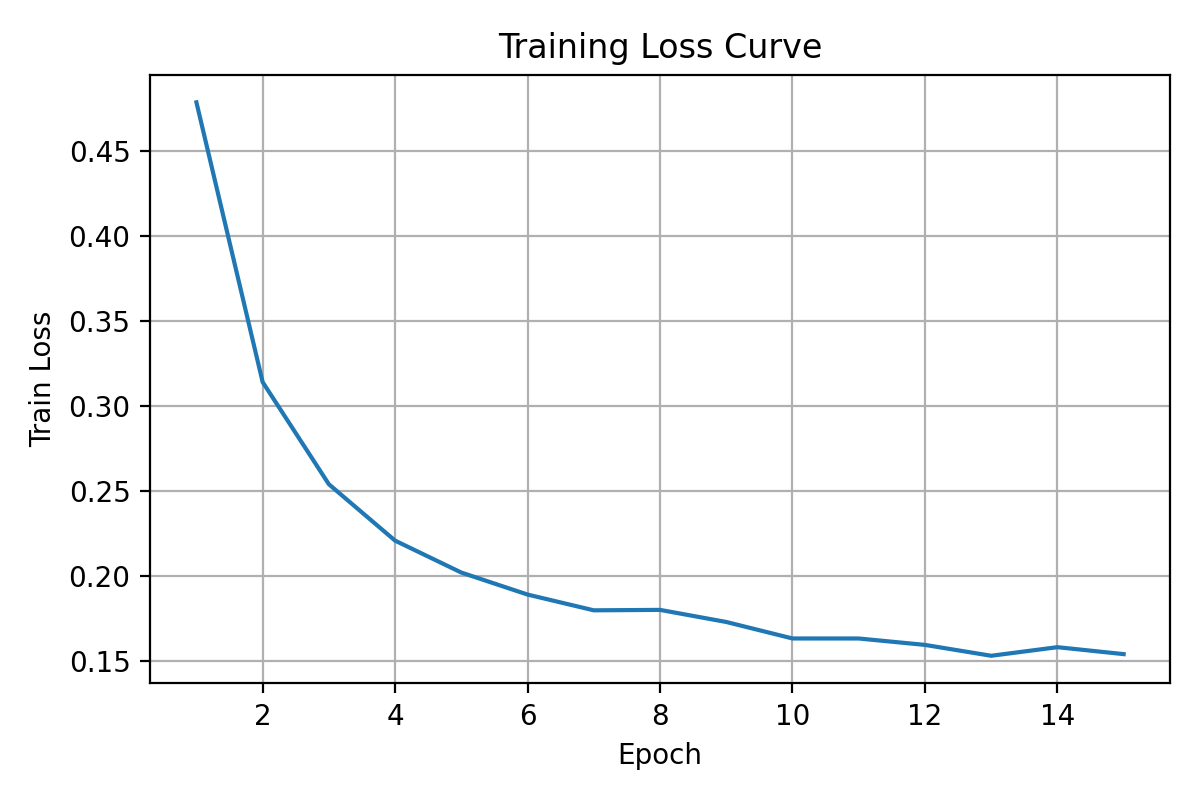
\includegraphics[width=0.85\linewidth]{figures/train_loss_curve.png}
\caption{Eğitim kaybının epoch'lara göre değişimi.}
\label{fig:trainloss}
\end{figure}

\begin{figure}[H]
\centering
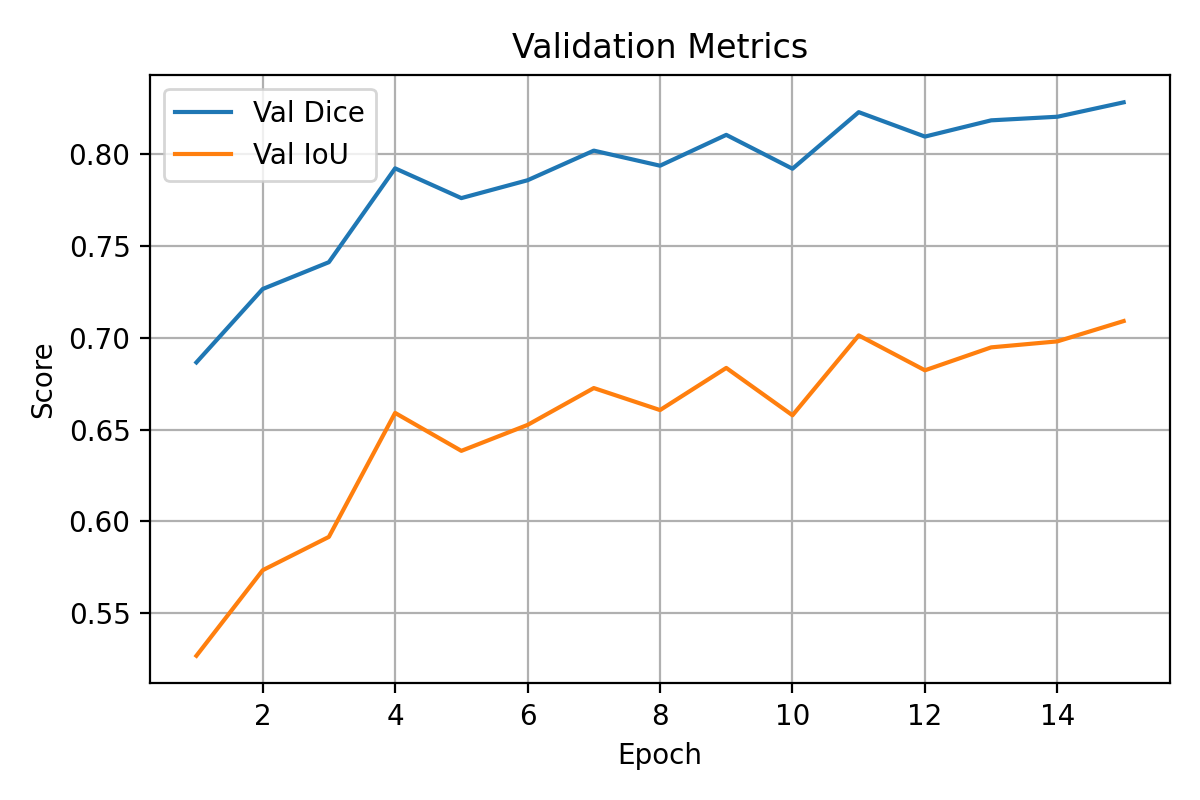
\includegraphics[width=0.85\linewidth]{figures/val_metrics_curve.png}
\caption{Doğrulama metriklerinin epoch'lara göre değişimi.}
\label{fig:valmetrics}
\end{figure}

\subsection{Nicel Test Performansı}
Test kümesinde (200 görüntü) görüntü başına ortalama (macro) metrikler Tablo~\ref{tab:test_macro}'te verilmiştir. Buna ek olarak, tüm test pikselleri üzerinde TP/FP/FN toplamları üzerinden hesaplanan piksel-ağırlıklı (micro) metrikler Tablo~\ref{tab:test_micro}'te sunulmuştur.

\begin{table}[H]
\centering
\small
\caption{Test kümesi macro metrikleri (mean$\pm$std).}
\label{tab:test_macro}
\begin{tabular}{lcc}
\toprule
\textbf{Metrik} & \textbf{Ortalama} & \textbf{Std. Sapma} \\
\midrule
Dice & 0.805876 & 0.075225 \\
IoU  & 0.680749 & 0.094570 \\
Precision & 0.809995 & 0.075987 \\
Recall & 0.808258 & 0.088333 \\
\bottomrule
\end{tabular}
\end{table}

\begin{table}[H]
\centering
\small
\caption{Test kümesi micro metrikleri (global TP/FP/FN üzerinden).}
\label{tab:test_micro}
\begin{tabular}{lc}
\toprule
\textbf{Metrik} & \textbf{Değer} \\
\midrule
Dice & 0.820165 \\
IoU  & 0.695152 \\
Precision & 0.816622 \\
Recall & 0.823739 \\
\bottomrule
\end{tabular}
\end{table}

\subsection{Nitel Sonuçlar}
Şekil~\ref{fig:qualitative} seçili örneklerde gerçek maske (GT), model tahmini ve hata karakterini (FP/FN) görsel olarak sunar. İyi performans gösteren örneklerin yanı sıra, ince damar uçlarında kaçırmaların (FN) belirginleştiği zor örnekler de raporlanmıştır.

\begin{figure}[H]
\centering
\small
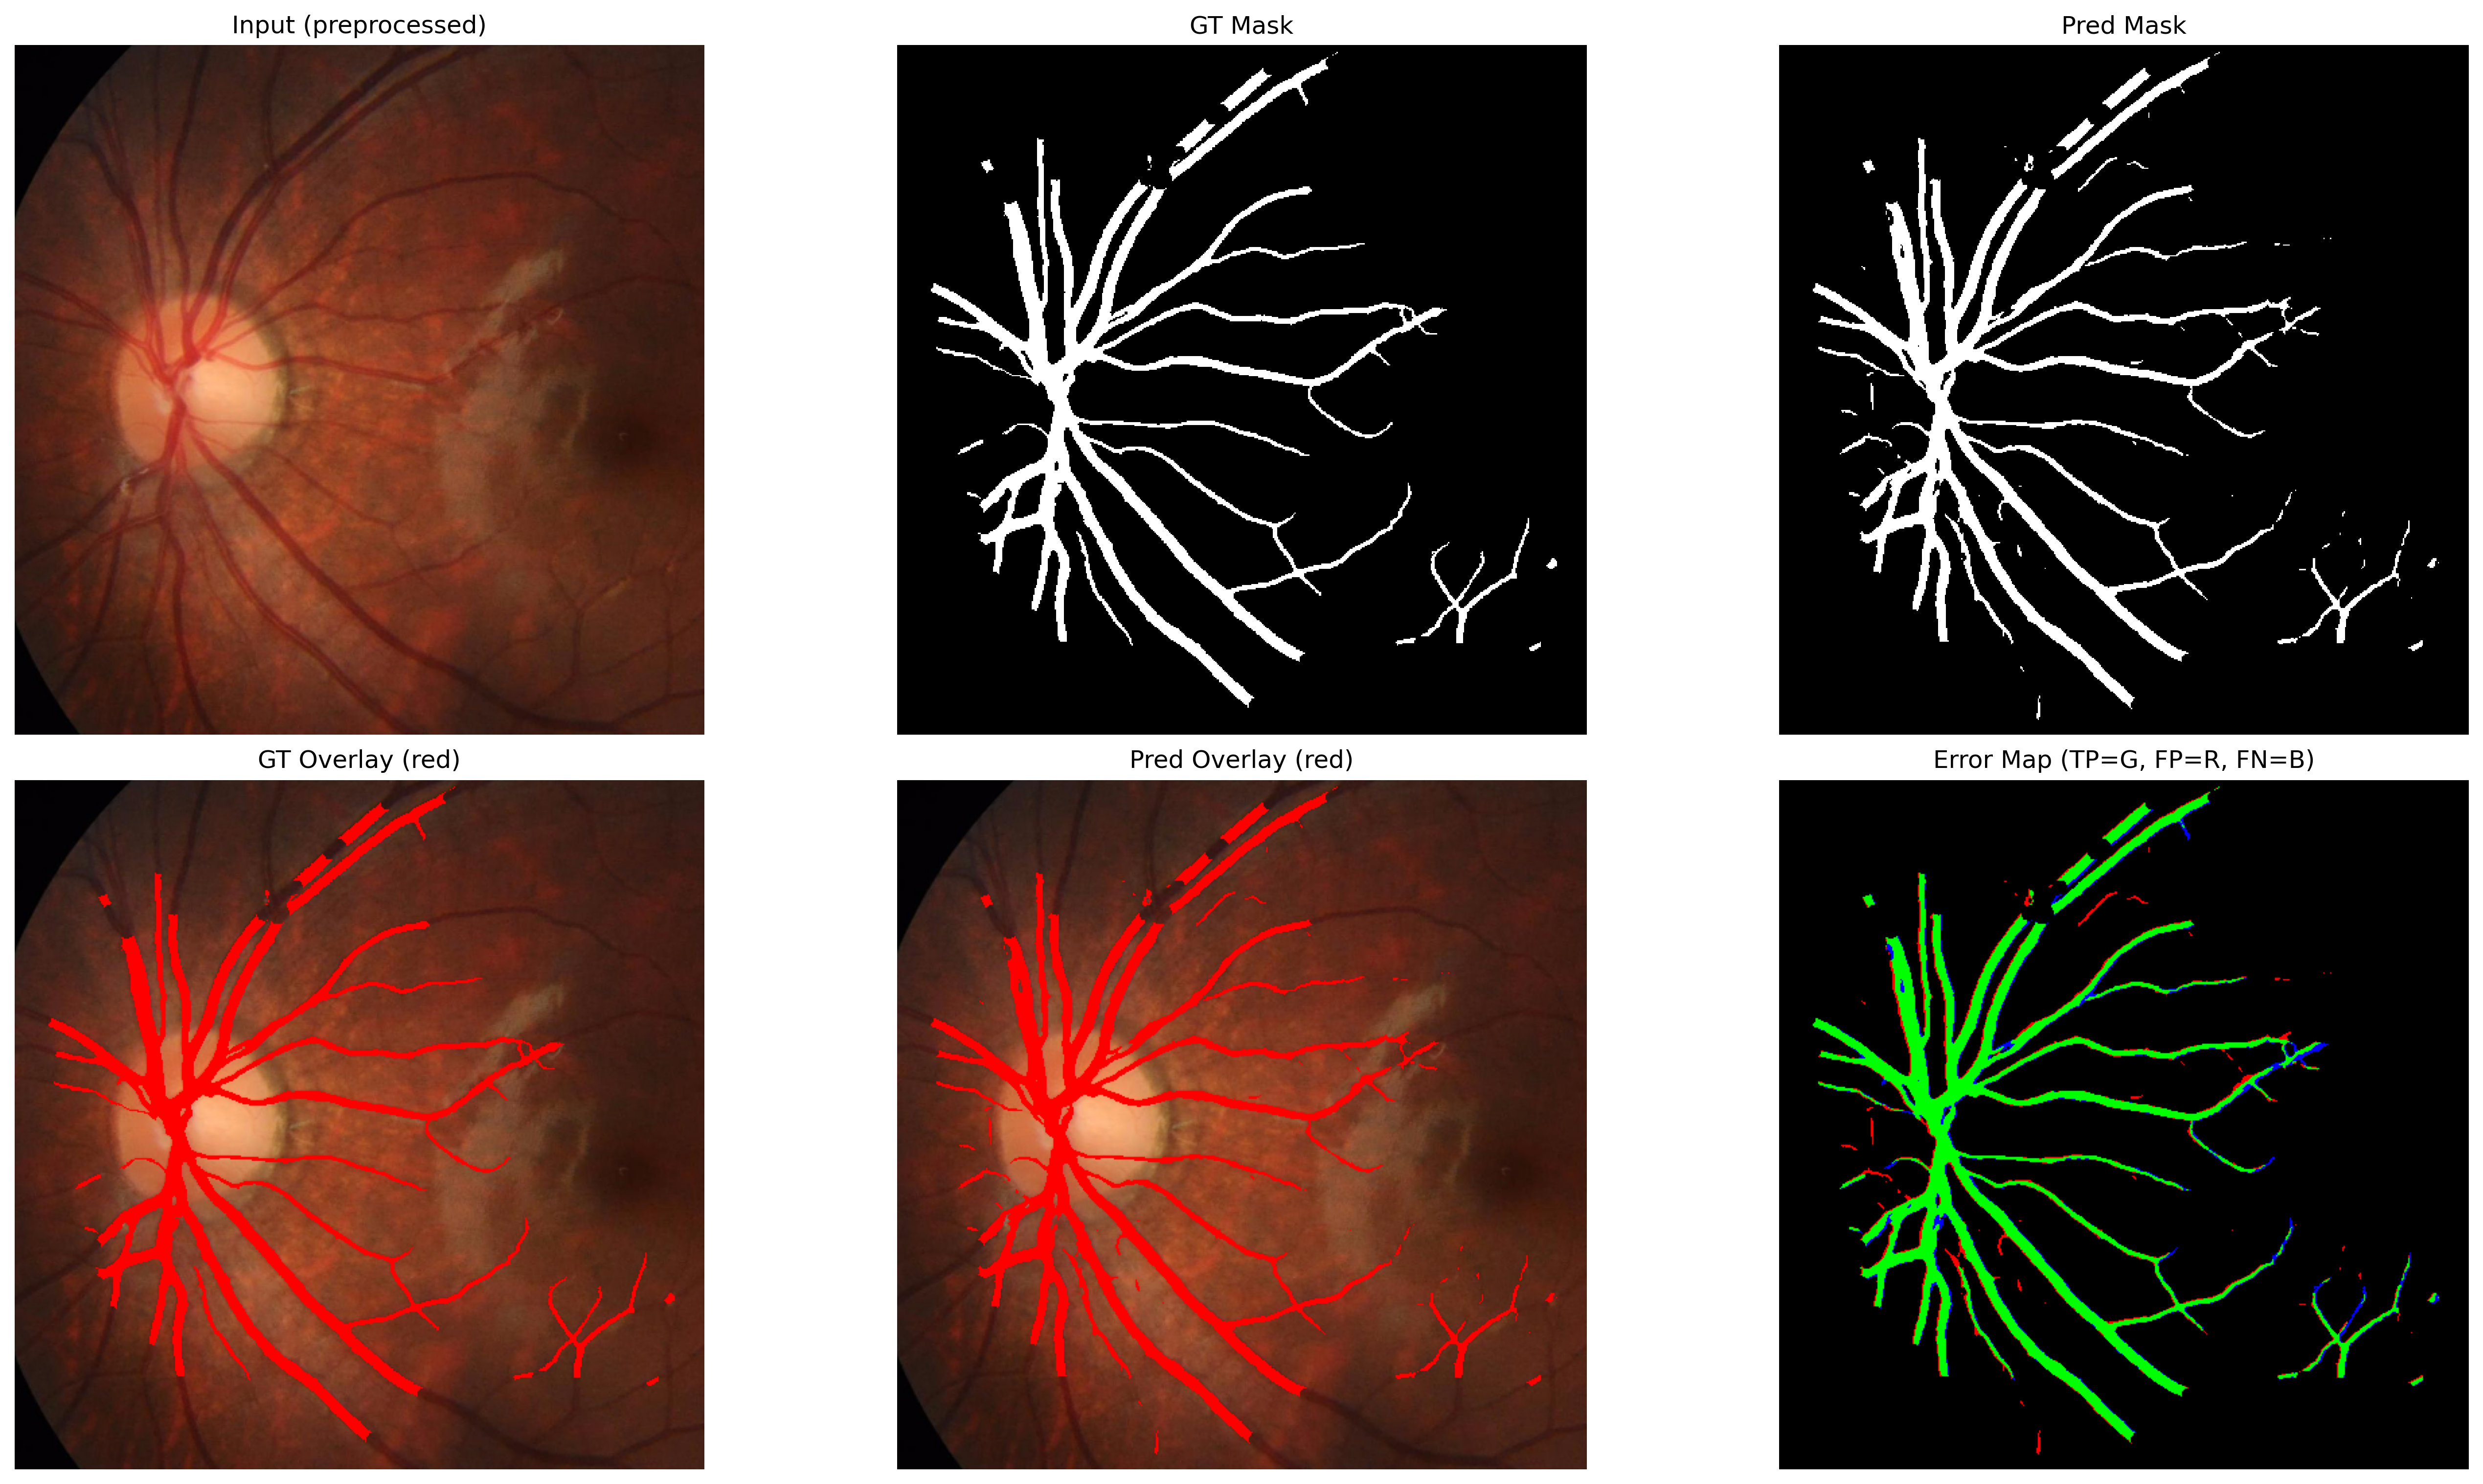
\includegraphics[width=0.48\linewidth]{figures/test_vis_160_N.png}\hfill
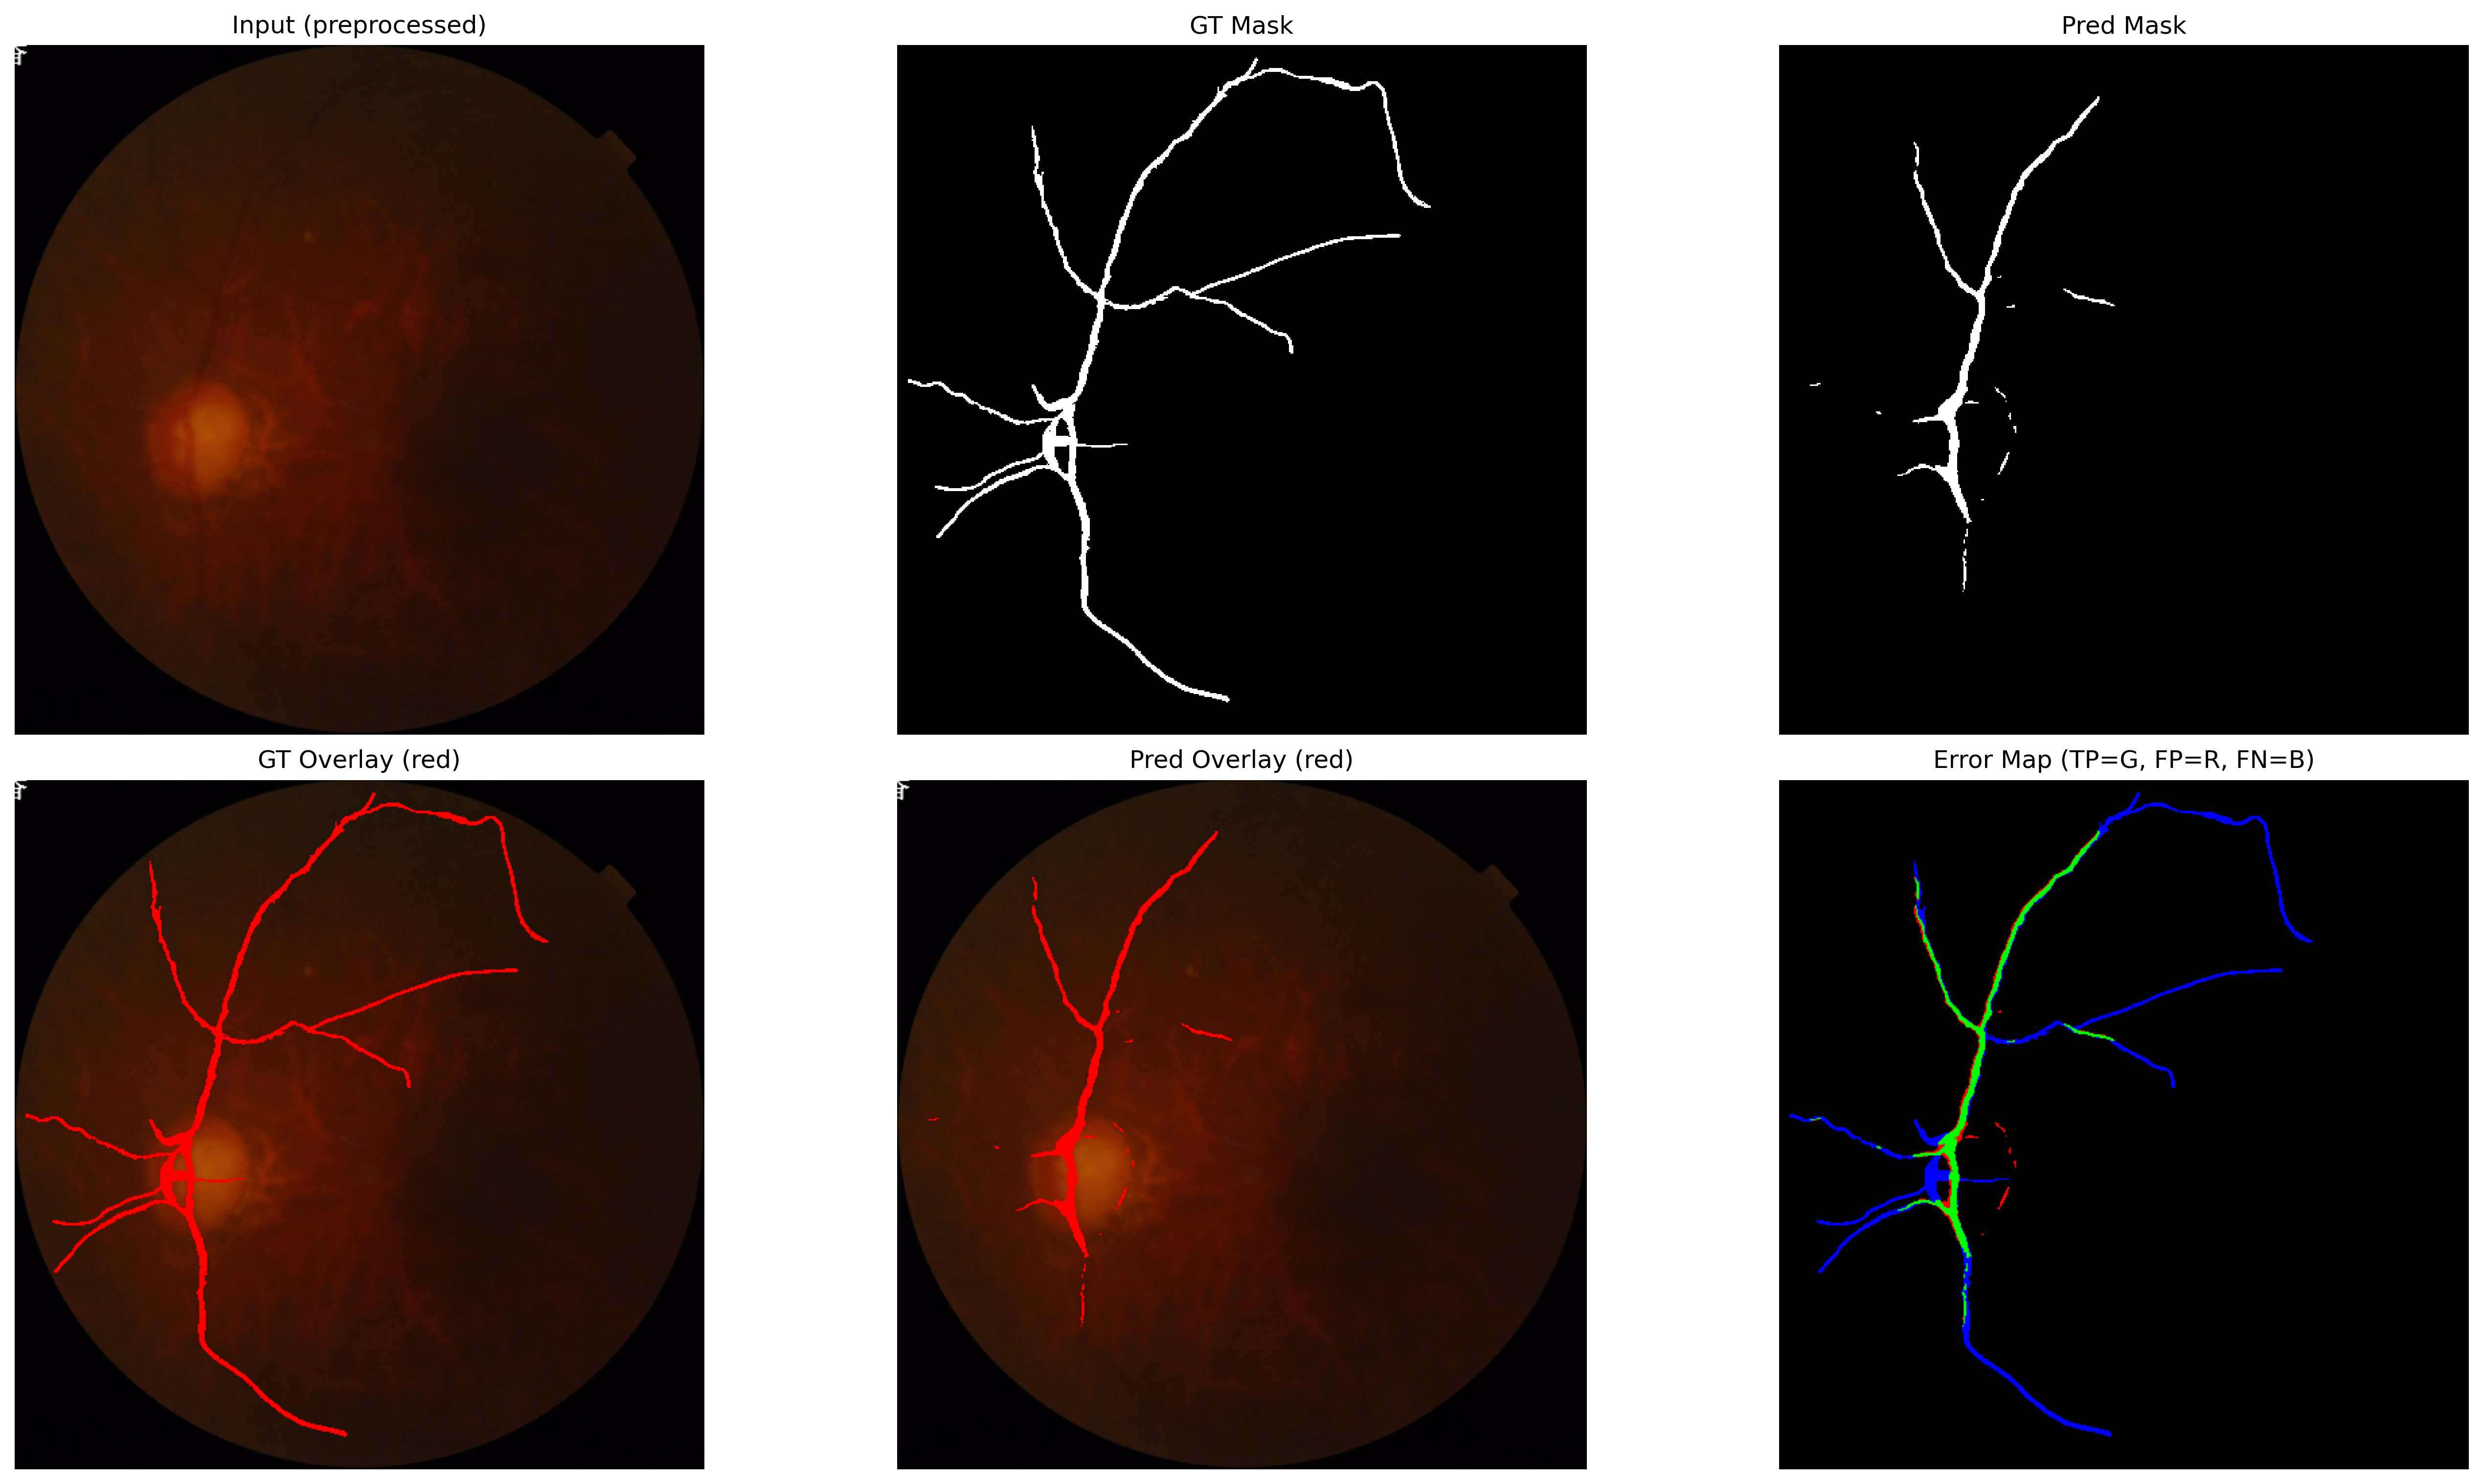
\includegraphics[width=0.48\linewidth]{figures/test_vis_136_G.png}\\
\vspace{0.5em}
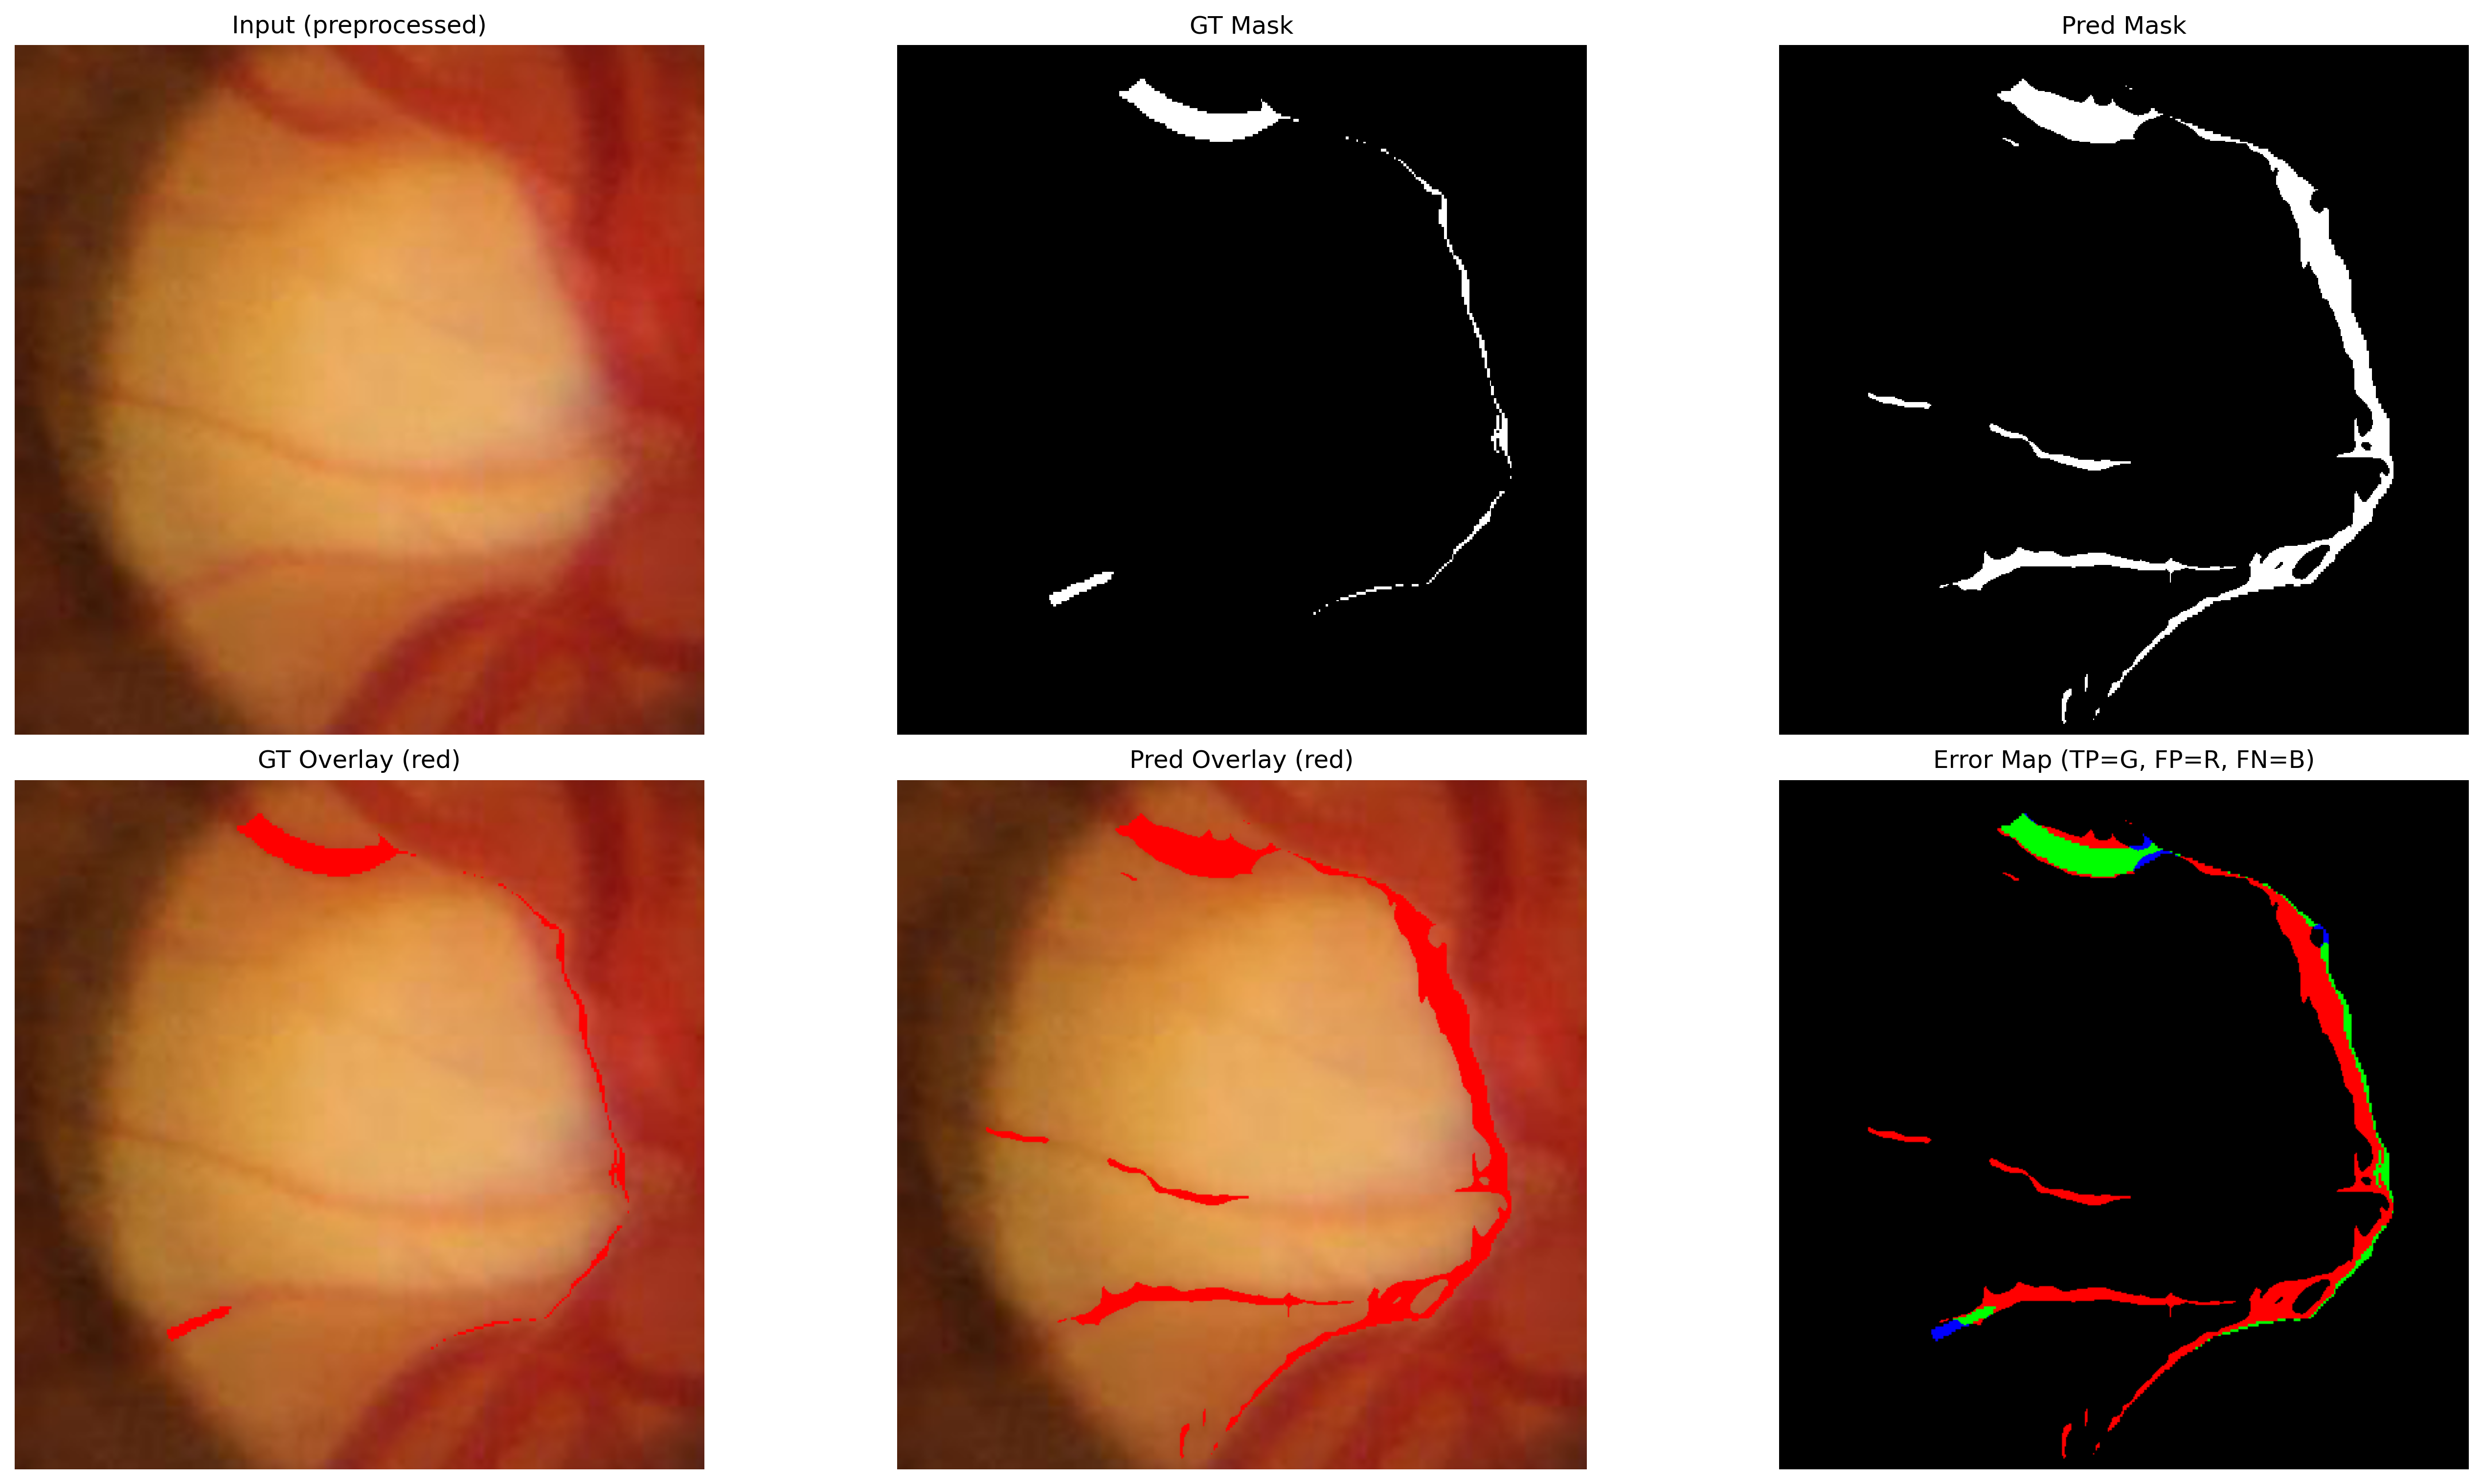
\includegraphics[width=0.48\linewidth]{figures/test_vis_112_G.png}\hfill
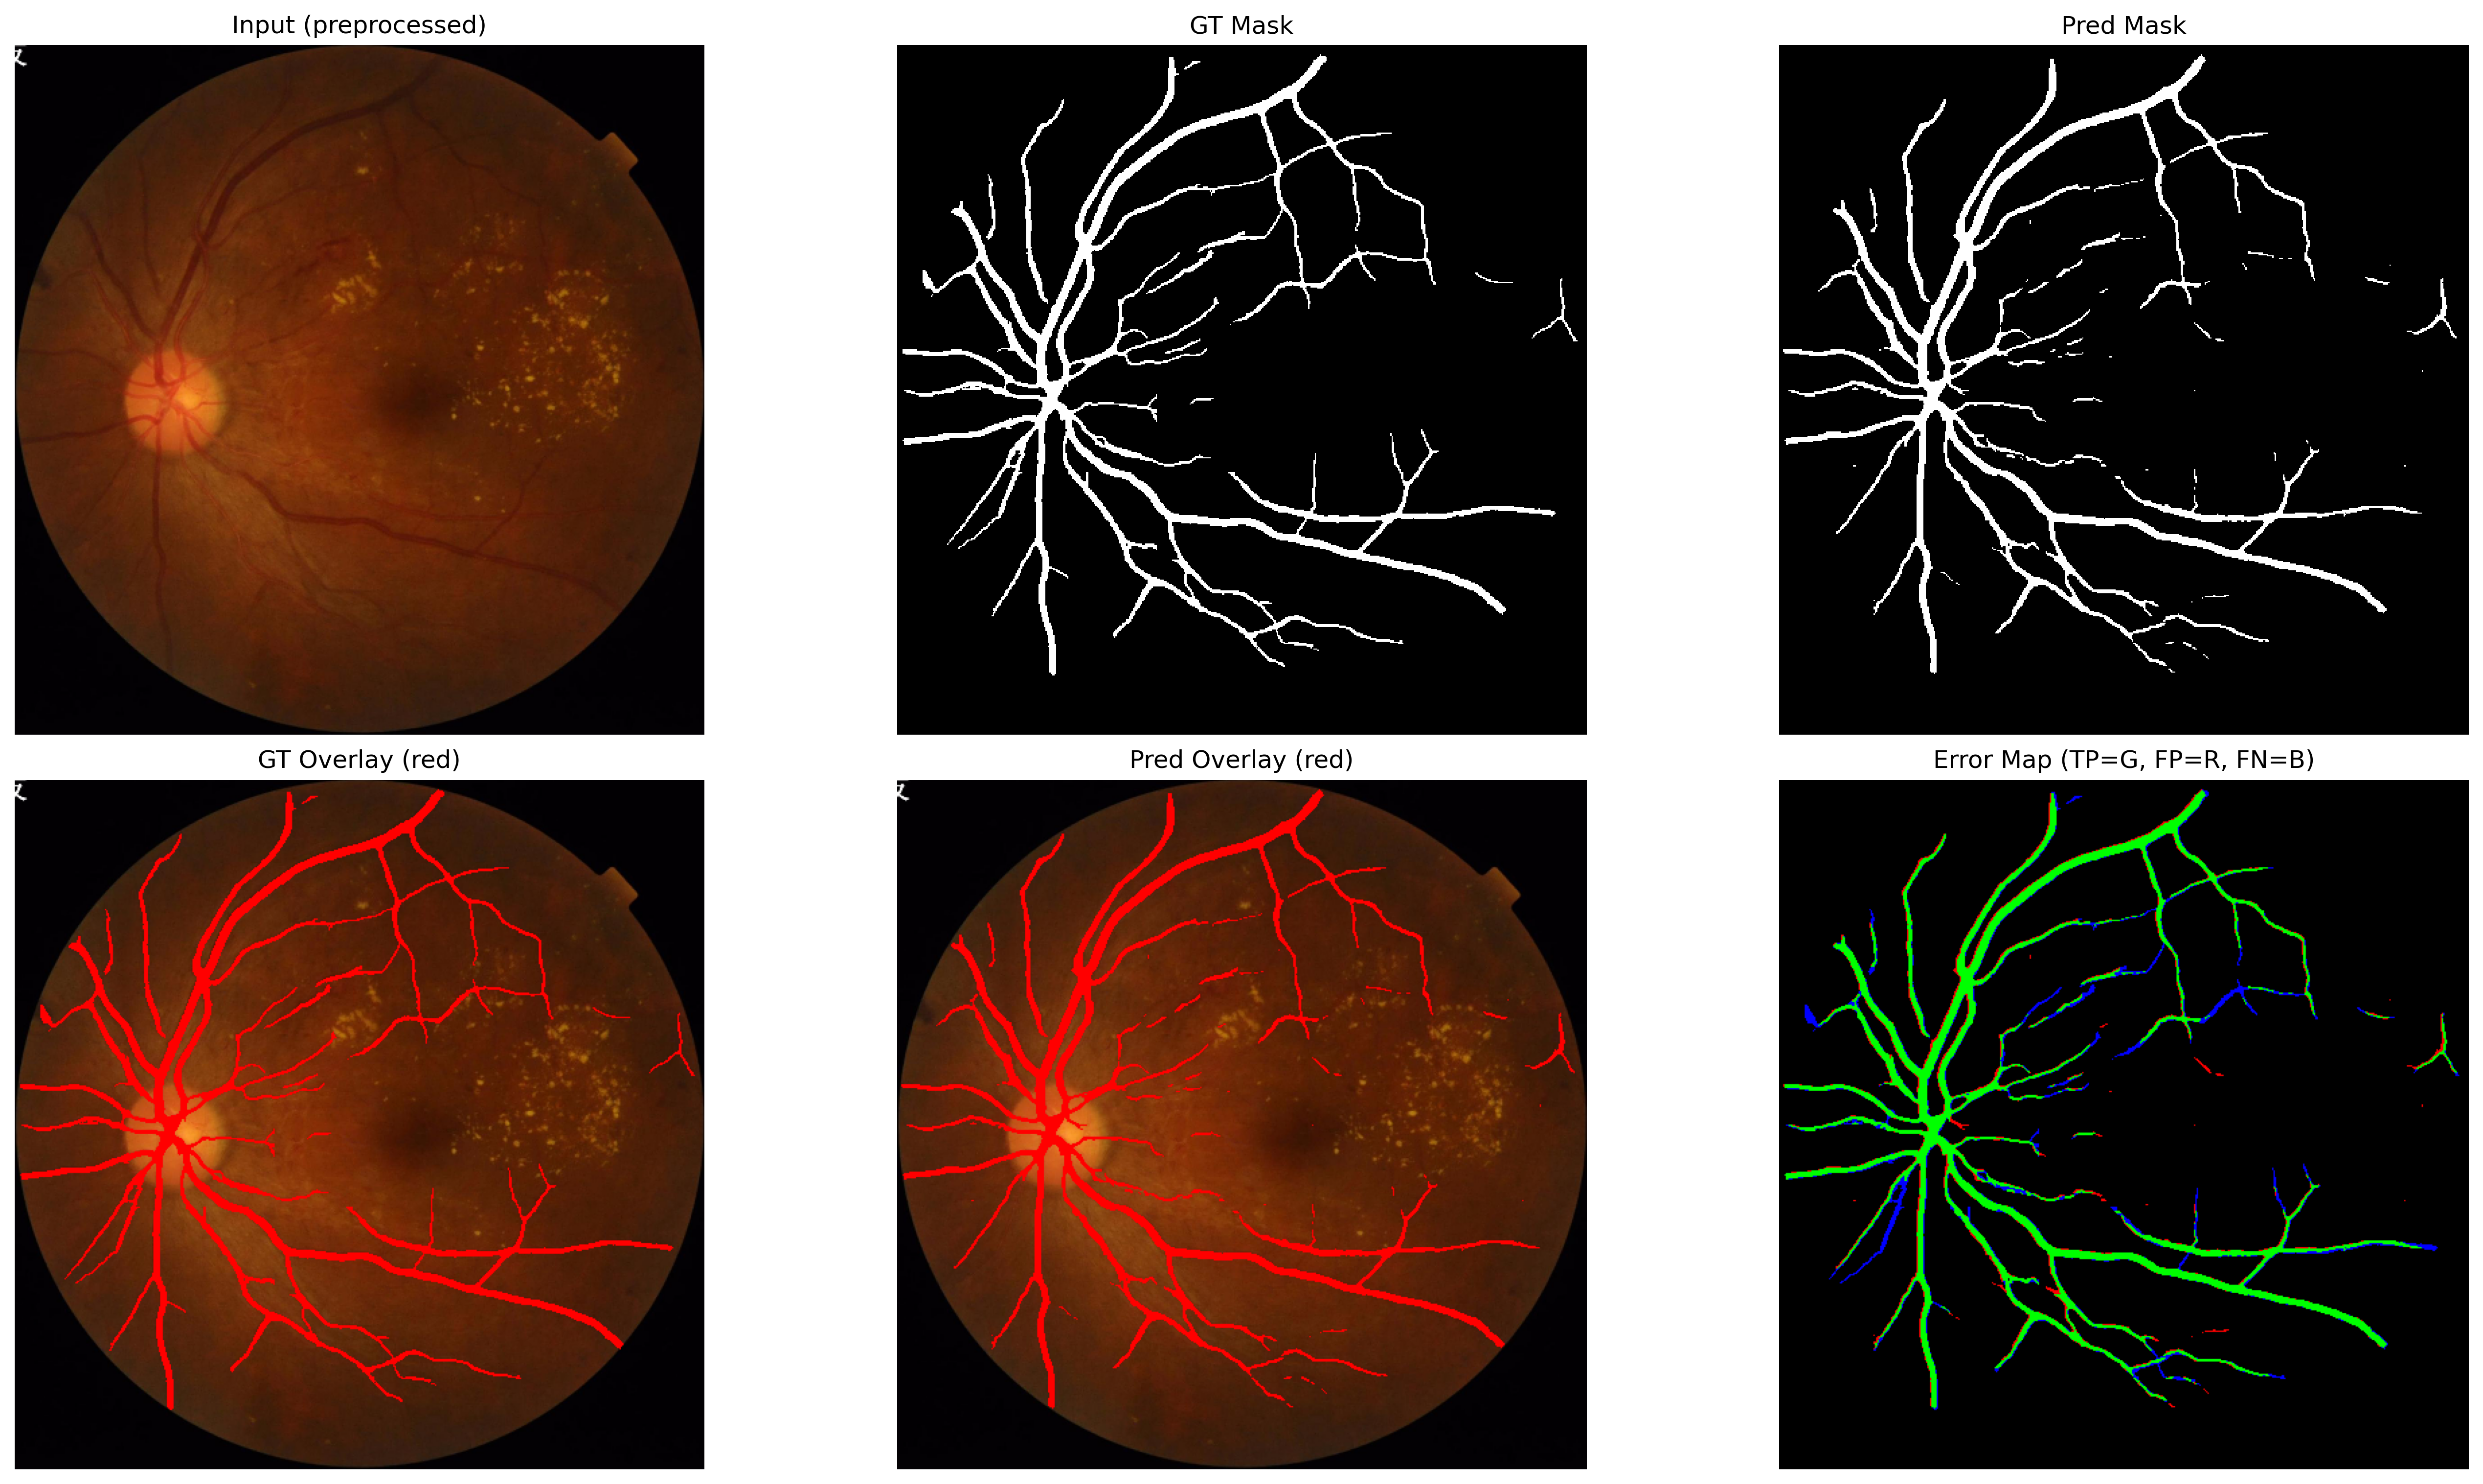
\includegraphics[width=0.48\linewidth]{figures/test_vis_90_D.png}
\caption{Seçili nitel örnekler: GT--tahmin karşılaştırmaları ve hata örüntüleri.}
\label{fig:qualitative}
\end{figure}

\subsection{Segmentasyon Sonrası Damar Analizi}
Segmentasyon çıktıları, damar yoğunluğu, iskelet uzunluğu ve dallanma sayısı açısından değerlendirilmiştir. Tablo~\ref{tab:vessel_analysis} sonuçları, damar yoğunluğunun ortalamada korunmasına karşın iskelet uzunluğu ve dallanma sayısında azalma eğilimi olduğunu göstermektedir.

\begin{table}[H]
\centering
\small
\caption{Damar analizi sonuçları (mean$\pm$std): GT ve model tahmini (Pred) karşılaştırması.}
\label{tab:vessel_analysis}
\begin{tabular}{lccc}
\toprule
\textbf{Gösterge} & \textbf{GT} & \textbf{Pred} & \textbf{Fark (Pred$-$GT)} \\
\midrule
Vessel density & $0.102824\pm0.039192$ & $0.103730\pm0.041278$ & $+0.000906\pm0.009618$ \\
Skeleton length (px) & $4830.675\pm1923.360$ & $4492.415\pm1730.630$ & $-338.260\pm452.431$ \\
Branch count & $277.445\pm139.570$ & $229.145\pm123.616$ & $-48.300\pm81.997$ \\
\bottomrule
\end{tabular}
\end{table}
